% ------------------------------Info--------------------------------
% Dieses Dokument ist als Vorlage f�r die studentischen Arbeiten
% am Institut f�r Thermodynamik gedacht. Es stellt eine einfache 
% M�glichkeit dar, die studentischen Arbeiten im Corporate Design
% der TU Braunschweig zu gestalten.
% Dazu wurden viele der notwendigen Einstellungen bereits in dieses
% Dokument eingearbeitet. Es steht dem Autor nat�rlich frei weitere
% Anpassungen, an seine individuellen kreativen Vorstellungen und 
% zum erfolgreichen Erstellen notwendigen Bed�rfnisse, vorzunehmen.
% Hierf�r sei an dieser Stelle auf die Website der Corporate Design
% (https://www.tu-braunschweig.de/presse/cd/toolbox) und die 
% Dokumentation zum Corporate Design in LaTeX hingewiesen.
%
% In diesem Sinne: Frohes Schreiben!
%-------------------------------------------------------------------

\documentclass[fontsize=11pt,
               paper=a4,	%Papierformat ist A4
               style=print, %[<print/printdev/screen>] Dokument ist f�r den Druck gedacht
               nexus, %Hausschrift der TU Braunschweig verwenden
               cmyk, % [<cmyk/rgb>]  Farben in CMYK Schema
               twoside=false, %Kein zweiseitiger Druck
               toc=bibliography ,%Literaturverzeichnis ohne Nummer im Inhaltsverzeichnis anzeigen
               blue % [<orange/blue/green/violet>] Farbschema f�r die Arbeit
              ]
              {tubsbook}
                       
%---------------------------------------------------
%---------------Allgemeine Angaben------------------
%---------------------------------------------------
\def \TITLE					{Adaptive Controller Design for Refrigeration Cycle Using the Natural Refrigerant  CO\textsubscript{2}}
\def \TYPE					{Masterarbeit} %[<Projektarbeit/Bachelorarbeit/Studienarbeit/Masterarbeit>]
\def \AUTHOR				{Julius Martensen}
\def \BETREUER				{Dipl. Ing. Michael N\"oding}
\def \TITELBILD				{pictures/Titelbild.png}
\def \AUFGABENSTELLUNG		{Aufgabenstellung.pdf}
\def \TOPLINE				{} %[<\showtopline>] % Aktiviert die rote Trennlinie �ber dem Bild. 
										%Sollte nur verwendet werden, wenn das Bild keine farbliche Trennung bietet.
%---------------------------------------------------
%----------Ende der Allgemeinen Angaben-------------
%
%		Header-Datei
%

% Nummerierungstiefe von section/subsection/subsubsection
\setcounter{secnumdepth}{3} 

%Absatzeinzug einstellen
\setlength{\parindent}{1em}
\setlength{\parskip}{0pt}

% Deutsche Rechtschreibung und deutscher Zeichensatz
\usepackage{german,ngerman}
\usepackage[ansinew]{inputenc}  

% Aktuelles Datum ermitteln
\usepackage[ngerman]{datenumber}

% Erweiterung f�r ein deutsches Literaturverzeichnis
\bibliographystyle{abbrvdin}

% Erweiterte Mathematikbibliotheken
\usepackage{amsmath}
\usepackage{amssymb}

% Ma�einhaeiten-Darstellung verbessern
\usepackage{units}

% Extra Symbole f�r die Verwendung im Text (z.B. \textcelsius)
%(werden nicht aus der Nexus-Schriftart einbunden)
\usepackage{textcomp}

% Einbinden von externen PDF Dateien
\usepackage[final]{pdfpages}

% Zum einbinden von Grafiken  
\usepackage{graphicx}
\usepackage{subcaption}  %erlaubt das erstellen von subfigures
\usepackage{float} %erm�glicht das erstellen von "non-floating figures"

%Hyperref f�r Verlinkungen im Dokument und URL's
%hyphens f�r verbesserten Zeilenumbruch in url's
\PassOptionsToPackage{hyphens}{url}
\usepackage[	breaklinks={true},
 						colorlinks	={true},
 					  	linkcolor	={tubsBlack},
  						citecolor	={tubsBlack},
  						filecolor	={tubsBlack},
  						urlcolor	={tuSecondaryMedium100},						
 					]{hyperref} %Interne Links in Schwarz und externe URL's in bg Farbe
 					
%Zus�tzliche Buchstaben und Zahlen erlauben f�r Zeilenumbruch bei url's (verbessert den Blocksatz)				
\expandafter\def\expandafter\UrlBreaks\expandafter{\UrlBreaks%  save the current one
  \do\a\do\b\do\c\do\d\do\e\do\f\do\g\do\i\do\j%
  \do\k\do\l\do\m\do\n\do\o\do\q\do\r\do\s%
  \do\u\do\v\do\w\do\x\do\y\do\z\do\A\do\B\do\C\do\D%
  \do\E\do\F\do\G\do\H\do\I\do\J\do\K\do\L\do\M\do\N%
  \do\O\do\P\do\Q\do\R\do\S\do\T\do\U\do\V\do\W\do\X%
  \do\Y\do\Z\do\1\do\2\do\3\do\4\do\5\do\6\do\7\do\8\do\9} 	
  
% R�ckseiten-Elemente
\address{% Addresse
  Technische Universit�t Braunschweig\\
  Institut f�r Thermodynamik\\
  Hans-Sommer-Strasse 5\\
  38106 Braunschweig}
\backpageinfo{}				

%Makro zur Formatierung des Anhangs
\newcommand{\Anhang}{
\appendix
\chapter*{Anhang}
\addcontentsline{toc}{chapter}{Anhang}
\setcounter{chapter}{1}
\markboth{Anhang}{Anhang}
\label{Anhang}}

%Makro zur Formatierung von der Titelseite bis zum Inhaltsverzeichniss
\newcommand{\Anfang}{
\pagenumbering{Roman}
\begin{titlepage}
%Designhelper f�r Erstellung 
%\showdesignhelper

\showtubslogo[right]
\showlogo{
\includegraphics{ift_4C.pdf}}
\TOPLINE

%Titelbild f�r die Arbeit
\begin{titlerow}[bgimage=\TITELBILD ,imagefit=cropped]{3}


\hfill\vfill
\end{titlerow}
\begin{titlerow}[bgcolor=tuSecondaryDark100, c]{2}

\begin{fitbox}{\textwidth}{100pt}
\raggedright
\color{tubsWhite}
\textbf{\TITLE}
\end{fitbox}
\addvspace{1,5em}
\begin{Large}
\raggedright
\color{tubsWhite}
\textbf{\TYPE}\vfill
\end{Large}

\end{titlerow}
\begin{titlerow}[bgcolor=tuSecondaryMedium80]{3}
\color{tubsWhite}


\begin{tabbing}
\hspace*{2.0cm}   \=  \hspace*{12.0cm}        \= \kill
\textbf{Autor:} \> \textbf{\AUTHOR} \\
\textbf{Betreuer:} \> \textbf{\BETREUER}\\
\textbf{Pr\"ufer:} \> \textbf{Prof. Dr.-Ing. J\"urgen K\"ohler}\\


 \> \textbf{\today}
\end{tabbing}
\hfill\vfill
\end{titlerow}
\hfill\vfill
\end{titlepage}

\includepdf[pages=-]{\AUFGABENSTELLUNG}
\addchap*{Eidesstattliche Erkl�rung}


\vspace*{5cm}


Hiermit erkl�re ich eidesstattlich, dass ich diese Arbeit eigenst�ndig angefertigt und keine anderen als die angegebenen Hilfsmittel verwendet habe.
\vspace{3cm}\\
Braunschweig den \today
\tableofcontents
\pagenumbering{arabic}
\setcounter{page}{1}}



%Makro zum einpassen des Titels in die Titelbox
\usepackage{environ}
\newdimen\fontdim
\newdimen\upperfontdim
\newdimen\lowerfontdim
\newif\ifmoreiterations
\fontdim12pt
\makeatletter
\NewEnviron{fitbox}[2]{% \begin{fitbox}{<width>}{<height>} stuff \end{fitbox}
  \def\buildbox{%
    \setbox0\vbox{\hbox{\minipage{#1}%
      \fontsize{\fontdim}{1.2\fontdim}%
      \selectfont%
      \stuff%
    \endminipage}}%
    \dimen@\ht0
    \advance\dimen@\dp0
  }
  \def\stuff{\BODY}% Store environment body
  \buildbox
  % Compute upper and lower bounds
  \ifdim\dimen@>#2
    \loop
      \fontdim.5\fontdim % Reduce font size by half
      \buildbox
    \ifdim\dimen@>#2 \repeat
    \lowerfontdim\fontdim
    \upperfontdim2\fontdim
    \fontdim1.5\fontdim
  \else
    \loop
      \fontdim2\fontdim % Double font size
      \buildbox
    \ifdim\dimen@<#2 \repeat
    \upperfontdim\fontdim
    \lowerfontdim.5\fontdim
    \fontdim.75\fontdim
  \fi
  % Now try to find the optimum size
  \loop
    %\message{Bounds: \the\lowerfontdim\space
    %         \the\fontdim\space \the\upperfontdim^^J}
    \buildbox
    \ifdim\dimen@>#2
      \moreiterationstrue
      \upperfontdim\fontdim
      \advance\fontdim\lowerfontdim
      \fontdim.5\fontdim
    \else
      \advance\dimen@-#2
      \ifdim\dimen@<10pt
        \lowerfontdim\fontdim
        \advance\fontdim\upperfontdim
        \fontdim.5\fontdim
        \dimen@\upperfontdim
        \advance\dimen@-\lowerfontdim
        \ifdim\dimen@<.2pt
          \moreiterationsfalse
        \else
          \moreiterationstrue
        \fi
      \else
        \moreiterationsfalse
      \fi
    \fi
  \ifmoreiterations \repeat
  \box0% Typeset content
}
\makeatother %Header zum Einbinden der Packages und zur Layout formatierung/konfiguration
\begin{document}
\Anfang

%---------------------------------------------------
%--------------Beginn eigener Kapitel---------------
%---------------------------------------------------
\chapter{Introduction}\label{c:intro}

\section{Motivation}\label{c:intro:s:motivation}

The great motivational Speak follows in this section.

\section{Literature Review}\label{c:intro:s:literature}

The great literature review follows in this section.
\chapter{Thermodynamic Model and\\ Problem Statement}\label{c:thermo}

The following chapter gives a brief introduction to the needed basics from a thermodynamic point of view.\\

In the first section the system is described from a technical perspective followed by  a general thermodynamic process model. \\

Afterwards the model used for simulating the system in Dymola is explained. \\

At last the problem motivating this thesis is formulated in the context of thermodynamics.


\section{Process Description} \label{c:thermo:s:process}

\section{Simulation Model Description} \label{c:thermo:s:sim}

\section{Problem Statement} \label{c:thermo:problem}
The aim of enginnering thermodynamics is - as stated earlier in Chap. \ref{c:intro} - to understand and optimize the  behaviour of technical systems used for energy transformation and transportation. Hence, a connection to the field of optimal control is a logical extension to maximize the efficiency. As described in sec. \ref{c:thermo:s:process} the systems states are general interconnected by both physical components and physical phenomena. In the following section the coupling due to physical phenomena will be investigated.\\

The process can be divided in three basic processes:
\begin{itemize}
\item Isobaric process with heat supply
\item Adiabatic isenthalpic process 
\item Isentropic process with exchange of (mechanical) work
\end{itemize}
We can characterize these processes using the First Law of Thermodynamics in differential form, see e.g. \cite[p.25]{Weigand2013ThermodynamikKompakt}:

\begin{align}
\begin{split}
du &= d \left( h - pv \right ) \\ &= dh - v dp - p dv \\
&= \delta q + \delta w_{diss} - p dv
\end{split}
\label{c:thermo:e:firstlaw}
\end{align}
\nomenclature{$u$}{Specific Inner Energy}
\nomenclature{$h$}{Specific Enthalpy}
\nomenclature{$p$}{Pressure}
\nomenclature{$v$}{Specific Volume}
\nomenclature{$q$}{Specific Heat}
\nomenclature{$w$}{Specific Work}

Which states that the change in inner energy $u \in \mathbb{R}$ is equal to the sum of heat $\delta Q \in \mathbb{R}$ and dissipated work $\delta w_{diss} \in \mathbb{R}$ minus the pressure-volume work, depending on the pressure $p \in \mathbb{R}^+$ times the change in specific volume $v \in \mathbb{R}^+$. The internal energy can be related to the specific enthalpy $h = u +pv \in \mathbb{R}$.\\

The Second Law of Thermodynamics as formulated by Gibbs \cite[p.59]{Struchtrup2014ThermodynamicsConversion} is given by:

\begin{align}
\begin{split}
T ds &= du + p dv \\
 &= d( h - pv ) + p dv \\
 &= dh - vdp
\end{split}
\label{c:thermo:e:secondlaw}
\end{align}
\nomenclature{$T$}{Temperature}
\nomenclature{$s$}{Specific Enthropy}

Defining two independent to be state variables the specific volume $v$ and temperature $T$ and substitute Eq.\ref{c:thermo:e:firstlaw} in Eq.\ref{c:thermo:e:secondlaw}:

\begin{align}
\begin{split}
T ds &= du + p dv \\
&= \delta q  + \delta w_{diss}
\end{split}
\label{c:thermo:e:firstandsecondlaw}
\end{align}

Since the total differential of the inner energy is given by


\begin{align}
\begin{split}
du &= \left( \frac{du}{dT} \right)_v dT  + \left( \frac{du}{dv} \right)_T dv
\end{split}
\label{c:thermo:e:innerenergydiff}
\end{align}

Substitute Eq. \ref{c:thermo:e:innerenergydiff} in \ref{c:thermo:e:firstandsecondlaw} while using the definition for the specific heat capacity at constant volume $c_V = \left(\frac{\partial u}{\partial T}\right)_v \in \mathbb{R}^+$ holds:

\begin{align*}
\begin{split}
T ds &= \left( \frac{\partial u}{\partial T} \right)_v dT  + \left( \frac{\partial u}{ \partial v} \right)_T dv + p dv \\
&= c_v dT + \left[ p + \left( \frac{\partial u}{\partial v}\right)_T\right] dv
\end{split}
\end{align*}

Using the relation \cite[p.375]{Struchtrup2014ThermodynamicsConversion} $T\left( \frac{\partial s}{\partial v}\right)_T = \left( \frac{\partial u}{\partial v}\right)_T + p $ and the Maxwell Relation $\left( \frac{\partial s}{\partial v}\right)_T = \left( \frac{\partial p}{\partial T}\right)_v = \frac{\beta}{\kappa} $ the equation becomes:

\begin{align}
\begin{split}
T ds &= \left( \frac{\partial u}{\partial T} \right)_v dT  + \left( \frac{\partial u}{ \partial v} \right)_T dv + p dv \\
\delta q &= c_v dT + T \frac{\beta}{\kappa} dv
\end{split}
\label{c:thermo:e:isobaricHeat}
\end{align}
\nomenclature{$c_v$}{Specific Heat Capacity at Constant Volume}
\nomenclature{$\beta$}{Coefficient of Thermal Expansion at Constant Pressure}
\nomenclature{$\kappa$}{Coefficient of Compressibility}

The coefficient of thermal expansion at constant pressure $\beta \in \mathbb{R}$ is defined by $\frac{1}{v}\left( \frac{dv}{dT} \right)_p = \beta$ and the compressibility $\kappa = \left( \frac{\partial v}{\partial p} \right)_T \in \mathbb{R}^+$ substitute the differential change of pressure due to temperature at constant volume via the chain rule.\newline

Eq. \ref{c:thermo:e:isobaricHeat} states that the exchange of heat in the isobaric process results in a change of specific volume and temperature. \\

The massflow $\frac{dm}{dt} = \dot{m} \in \mathbb{R}$ from A to B through a throttle can be described by a function of the density $\rho = \frac{1}{v} \in \mathbb{R}^+$, the effective area $A_{eff} \in \mathbb{R}^+$ and the difference in pressure 

\begin{align}
\begin{split}
\dot{m} & = A_{eff} \sqrt{2 \rho_A  \left( p_A -p_B \right) }
\end{split}
\label{c:thermo:e:throttle}
\end{align}
\nomenclature{$A_{eff}$}{Effective Area}
\nomenclature{$\rho$}{Density , Specific Mass}
\nomenclature{$\dot{m}$}{Massflow}

we can directly relate the difference pressure $p_A - p_B = \Delta p > 0$ to the exchange of heat. Assume a constant mass flow, a constant effective Area and a constant pressure niveau $p_B$ due to perfect controller of the system, the energetic coupling between fan and pressure can be seen. If heat is added before A as described by Eq. \ref{c:thermo:e:isobaricHeat} the Temperature in A will be influenced as well the pressure due to the change in the specific volume and therefore the density via Eq.\ref{c:thermo:e:throttle}.\\

The isenthalpic, adiabat throttling process can be described by the Joule-Thomson Coefficient \cite[p.387]{Struchtrup2014ThermodynamicsConversion}. The equation relates the change in temperature and pressure to each other via

\begin{align}
\begin{split}
\left( \frac{\partial T}{\partial p}\right)_h &= -\frac{1}{c_p} \left(\frac{\partial h}{ \partial p} \right)_T \\
&= \frac{v}{c_p}\left( T\beta - 1 \right) 
\end{split}
\label{c:thermo:e:joulethomson}
\end{align}

Where $c_p = \left(\frac{\partial h}{\partial T} \right)_p \in \mathbb{R}^+$ is the specific heat at constant pressure which relates the change in entropy due to a change in temperature.
Eq. \ref{c:thermo:e:joulethomson} and Eq. \ref{c:thermo:e:throttle} relate the change in pressure via variation of the effective Area to the change in temperature. \\

Eq. \ref{c:thermo:e:isobaricHeat}, \ref{c:thermo:e:throttle} and \ref{c:thermo:e:joulethomson} show the thermodynamic coupling of the system. They are highly nonlinear and give an ideal coupling for the quasi stationary processes and the choosen states pressure and temperature. Since both couplings take effect at the same time, a reasonable estimation of the process trajectory is difficult.\newline
An important fact is that none of the equations above depend explicitly on the time. All coefficients above are functions of the thermodynamic states $p,v,T,s$. Assuming quasi stationary behaviour of the system for every coefficent $c \in \left\lbrace \beta, \kappa, c_v, c_p \right\rbrace$ they can be related to the static gain of the couplings.\\

Further physical phenomena interconnecting the system can be related to hydraulic capacity, hydraulic inductivity 
\chapter{Control Theoretic Model and Problem Statement}\label{c:control}

The following chapter explains the 

\section{Basics of Control Theory}\label{c:control:s:basics}

A general nonlinear, dynamical system $\Sigma$ can be described \cite{Adamy2014}

\begin{align}
\begin{split}
\ve{\dot{x}} &= \ve{f}\left(\ve{x},\ve{u}, t\right) \\
\ve{y} &= \ve{h}\left(\ve{x},\ve{u},t \right)
\end{split}
\label{c:control:e:nonlinearsystem}
\end{align}
\nomenclature{$\ve{x}$}{State Vector of a Dynamical System}
\nomenclature{$\ve{u}$}{Input Vector of a Dynamical System}
\nomenclature{$\ve{y}$}{Output Vector of a Dynamical System}
\nomenclature{$\ve{f}$}{Vector Function of a Nonlinear Dynamical System}
\nomenclature{$\ve{h}$}{Output Vector Function of a Nonlinear Dynamical System}


Where $t \in \mathbb{R}^+$ is the time, $\ve{x} \in \mathbb{R}^{n_x}$ is called the state vector, or states, and $\ve{u} \in \mathbb{R}^{n_u}$ the input vector, or inputs, of the system. The output $\ve{y} \in \mathbb{R}^{n_y}$ of the system is described by the functions$\ve{h}~:\mathbb{R}^{n_x},\mathbb{R}^{n_u},\mathbb{R}^+ \mapsto \mathbb{R}^{n_y}$ and the evolution of the system over time is given by $\ve{f}:~\mathbb{R}^{n_x},\mathbb{R}^{n_u},\mathbb{R}^+ \mapsto \mathbb{R}^{n_x} $.\\

The System given by Eq. \ref{c:control:e:nonlinearsystem} can be used to describe almost every natural or technical system.\newline
Due to several reasons, e.g. controller design, measurements, modelling issues and errors, most technical applications simplify the model by assuming linear, time invariant (LTI) behaviour. The LTI system is represented by a set of first-order differential equations \cite{Lunze2014} called state space representation:

\begin{align}
\begin{split}
\ve{\dot{x}} &= \ma{A}~\ve{x} + \ma{B}~\ve{u} \\
\ve{y} &= \ma{C}~\ve{x} + \ma{D}~\ve{u}
\end{split}
\label{c:control:e:ltisystem}
\end{align}
\nomenclature{$\ma{A}$}{State Matrix of a Dynamical System}
\nomenclature{$\ma{B}$}{Input Matrix of a Dynamical System}
\nomenclature{$\ma{C}$}{Output Matrix of a Dynamical System}
\nomenclature{$\ma{D}$}{Feedthrough Matrix of a Dynamical System}
The state matrix $\ma{A} \in \mathbb{R}^{n_x\times n_x}$ describes the influence of the current states, the input matrix $\ma{B} \in \mathbb{R}^{n_x\times n_u}$ the influence of the current input on the future states and output. The output is given by the output matrix $\ma{C} \in \mathbb{R}^{n_y\times n_x}$ and the feedthrough matrix $\ma{D} \in \mathbb{R}^{n_y\times n_u}$.\\

Both Eq. \ref{c:control:e:nonlinearsystem} and Eq. \ref{c:control:e:ltisystem} are able to generate a variety of different controllers, see e.g. \cite{Adamy2014},\cite{Lunze2014}, \cite{Lunze2016}. The ability to design controller via state space methods is connected to a high information content about (physical) parameters and equations or in form of measurement data.\\

Hence a more compressed form is commonly used to design controller for most technical and industrial applications. The transfer function matrix \cite[p.20]{Lunze2014} $\ma{G} \in \mathbb{C}^{n_y\times n_u}$ can be derived via the Laplacetransform of Eq.\ref{c:control:e:ltisystem}:

\begin{align}
\begin{split}
\ma{G} &= \ma{C} \left(s \ma{I} - \ma{A} \right)^{-1} \ma{B} + \ma{D} \\
\end{split}
\label{c:control:e:TransferFunctionMatrix}
\end{align}
\nomenclature{$\ma{G}$}{Transfer Function Matrix}

The transfer function matrix consist of single transfer functions $g_{ij}(s)~, i \leq n_y, j \leq n_u$ and maps the transformed input of a system directly to its  transformed output. It describes the relationship between input and output directly and is hence a compact form of describing the behaviour of LTI systems. To control a system with two outputs in every wanted direction a necessary condition is given by $n_y \leq n_u$. It is assumed that all following systems suffice $\dim{\ma{G}} = n_y \times n_y$.  \\

\section{Feedback Control in Presence of Uncertain Signals}

The aim of control theory is to manipulate a systems trajectory via its inputs in such a way, that a desired output is reached and maintained. To do this, several techniques can be used. Most commonly the systems desired output, the setpoint $\ve{y}_r$, is compared to the actual output of the system $\ve{y}$ via a feedback loop. The result of this comparison is called the error $\ve{e} \in \mathbb{R}^{n_y}$ \nomenclature{$\ve{e}$}{Error Signal of a Feedback Loop}. This signal is fed into the controller $\ma{K} \in \mathbb{C}^{n_y \times n_y}$ \nomenclature{$\ma{K}$}{Controller of a Dynamical System} and the result is used as an input for the system. This approach is called feedback control, see e.g. \cite{Astrom2009FeedbackEngineers}, with a single degree of freedom controller.\\

A variation of this approach is to use a weighted set point and output signal to generate the input. The pair of weighting matrices $\ma{K}_r$  for the setpoint and $\ma{K}_y$ for the output is called a two degree of freedom controller. The structure of such a controller design is shown in Fig. \ref{c:control:f:2dofclosedloop}.

\begin{figure}[H]
\begin{minipage}[b]{\textwidth}
\centering
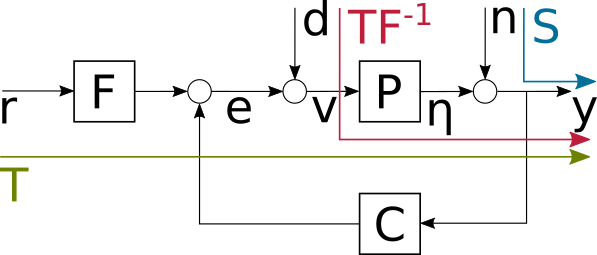
\includegraphics[width=0.9\textwidth]{./Graphics/2DOFCLOSEDLOOP.png}
\caption{Two Degree of Freedom Feedback Control}
\label{c:control:f:2dofclosedloop}
\end{minipage}
\end{figure}

In Fig. \ref{c:control:f:2dofclosedloop} other signals are added as well.The disturbances $\ve{d} \in \mathbb{R}^{n_y}$ are acting on the weighted error. The signal $\ve{v} \in \mathbb{R}^{n_y}$ is the disturbed input of the plant. $\ve{\eta} \in \mathbb{R}^{n_y}$ is the plants output without measurement noise which will be referred to as real output. The measurement noise is given by $\ve{n} \in \mathbb{R}^{n_y}$. The superposition of noise and real output is $\ve{y}$ which will be referred to simply as output. The closed loop transfer function is given by:

\begin{align}
\begin{split}
\ve{y} &= \left[\ma{I} - \ma{G} \ma{K}_y\right]^{-1} \left[ \ma{G}\ma{K}_r \ve{y}_r + \ve{n} + \ma{G} \ve{d} \right]
\end{split}
\label{c:control:e:2dofclosedloop}
\end{align}
\nomenclature{$\ve{d}$}{Disturbance Vector of a Dynamical System}
\nomenclature{$\ve{n}$}{Measurement Noise Vector of a Dynamical System}

Eq. \ref{c:control:e:2dofclosedloop} relates the output of a system to the influences of set point, disturbances and measurement noise. 
Rewriting the equation as:

\begin{align}
\begin{split}
\ve{y} &= \ma{T}\ve{y}_r + \ma{S} \left[ \ve{n} + \ma{G} \ve{d} \right]
\end{split}
\label{c:control:e:sensitivityclosedloop}
\end{align}
defines the Sensitivity Function $\ma{S} = \left[ \ma{I} - \ma{G} \ma{K}_y\right]^{-1} \in \mathbb{C}^{n_y \times n_y}$ which relates the influences of measurement noise and load disturbance to the systems outputs. The Complementary Sensitivity Function $\ma{T} = \left[\ma{I} - \ma{G} \ma{K}_y\right]^{-1} \ma{G} \ma{K_r} \in \mathbb{C}^{n_y \times n_y}$ describes the response to the reference signal.Both Functions play an important role in the investigation of the systems Robustness and are connected to each other via $\ma{T} = \ma{S} \ma{G} \ma{K}_r$.\\

\section{Robustness and Stability of Feedback Control Systems}

Robustness refers in general to the stability of the system in presence of uncertainties and has been studied extensively, see e.g. \cite{Zhou1998EssentialsControl},\cite{Zhou1996RobustControl}, \cite{DoyleFeedbackTheory}.
To give a better understanding of the relevant points of the subject both SISO and MIMO cases are presented. \\

For any given SISO system with a transfer function $g : \mathbb{R} \mapsto \mathbb{C}$ we see from Eq. \ref{c:control:e:2dofclosedloop} that the behaviour of the output with respect to measurement noise and disturbances is strongly dependent on the sensitivity function. A necessary condition for the system to reach the reference is that disturbance and noise are attenuated  near the steady state. Furthermore the destabilizing effect due to uncertain signals can be quantified via the maximum of the sensitivity function. Therefore the Maximum Sensitivity is defined as:

\begin{align}
\begin{split}
M_S & = \max_\omega \left| S \right| \\
& \geq \left| \frac{1}{1 - g~k_y}\right|
\end{split}
\label{c:control:e:maxsensitivity}
\end{align}

With Eq. \ref{c:control:e:maxsensitivity} an upper boundary on the gain can be found and be used as a measure of robustness of the closed loop \cite[p.323 ff.]{Astrom2009FeedbackEngineers}. The maximum sensitivity is also connected to the nyquist stability and the stability margin of a system via:

\begin{align}
\begin{split}
M_S &= \frac{1}{s_M} \\
&= \frac{1}{1 - \max_\omega \left| g ~k_y \right|}
\end{split}
\label{c:control:e:maxsensitivitynyquist}
\end{align}

Or rearranged to be:

\begin{align}
\begin{split}
\max_\omega \left| g~k_y\right| &= 1 - s_M
\end{split}
\end{align}

Due to Eq. \ref{c:control:e:maxsensitivitynyquist} the maximum gain of the open loop is limited by the maximum sensitivity. Hence, the critical point is only encircled iff the maximum sensitivity is zero. Hence the system is only stable in the sense of the Nyquist Criterion if the maximum sensitivity is sufficiently small.\\

\begin{figure}[H]
\begin{minipage}[b]{\textwidth}
\centering
\input{./Graphics/MS.pdf_tex}
\caption{Maximum Sensitivity}
\label{c:control:f:MaximumSensitivity}
\end{minipage}
\end{figure}


While the maximum sensitivity is well definied for SISO systems, a MIMO system requires a more general approach due to the interconnection of the systems out- and inputs. A general condition is given by the Small Gain Theorem \cite[p.150 ff.]{Skogestad2005MultivariableDesign}. The theorem states, that a given feedback system is stable iff the open loop transfer function matrix is stable and its sufficient conditioned matrix norm is less than 1 over all frequencies.

\begin{align}
\lVert \ma{G} \ma{K}_y \rVert < 1 ~\forall \omega
\label{c:control:e:SmallGainTheorem}
\end{align}

Eq. \ref{c:control:e:SmallGainTheorem} can be used with several matrix norms and can be viewed as an MIMO Interpretation of the Nyquist Criterion. \\

For further robustness analysis, the concept of singular values has to be investigated. The singular value decomposition, see e.g. \cite[p.144 f.]{2013Springer-HandbuchIII},states that any matrix $\ma{G} \in \mathbb{C}^{n_a\times n_b}$ can be factorized such that

\begin{align}
\ma{G} &= \ma{U}\ma{\sigma}\ma{V}^*
\label{c:control:e:SVD}
\end{align}

Where as $\ma{U} \in \mathbb{C}^{n_a \times n_a}$ and $\ma{V} \in \mathbb{C}^{n_b \times n_b} $ are unitary matrices representing the left and right eigenvectors of matrix. The matrix $\ma{\sigma} \in \mathbb{C}^{n_a \times n_b}$ is a rectangular, diagonal matrix consisting of the singular values $\sigma \in \mathbb{C}$ of $\ma{G}$. A practical point of view suggest a rotation of any given input vector via $\ma{V}^*$, distributing the magnitude of the input over the columns of $\ma{\sigma}$, where they are scaled according to the magnitude of the corresponding singular value. Then the scaled and rotated vector is once again rotated by $\ma{U}$ and distributed over the output vector. \\

\begin{figure}[H]
\begin{minipage}[b]{\textwidth}
\centering
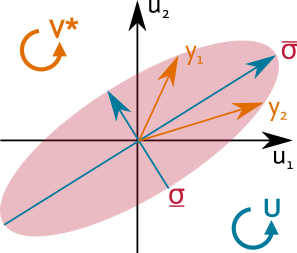
\includegraphics[scale=1]{./Graphics/SVD.png}
\caption{Graphical Interpretation of the Singular Value Decomposition}
\label{c:control:f:SVD}
\end{minipage}
\end{figure}



An example of this process is illustrated in Fig. \ref{c:control:f:SVD} for a system with two inputs $u_1,u_2$ and two outputs $y_1,y_2$. The output is bounded by the ellipsoid described by the maximum singular value $\overline{\sigma}$ and the minimum singular value $\underline{\sigma}$. The orientation and the magnitude of the outputs change depending on the frequency but will never exceed these limits. The singular values of a matrix are hence representing the highest possible gain for any given input if $\ma{U} = \ma{V}^* = \ma{I}$. With that, the induced 2-Norm for a matrix can be defined as:

\begin{align}
\begin{split}
\lVert \ma{G} \rVert_2 &= \frac{\lVert \ma{G}\ma{u}\rVert_2}{\lVert \ma{u} \rVert_2} \\
&= \max \sqrt{\lambda\left( \ma{G}^* \ma{G}\right)} \\
&= \overline{\sigma}
\end{split}
\label{c:control:e:MaxSingularValue}
\end{align}

\section{System Identification of Dynamical Processes}\label{c:control:s:identification}

For controlling a system as given earlier, knowledge about the dynamics of the system is used. While physical models can be used to derive a controller, not every effect and not every physical parameter is known perfectly. Hence a physical model is not always an appropriate basis for designing a controller fit for the task.\\

With respect to the specific problem at hand, one can easily imagine the difference in the dynamics of the system due to a change of parameters like length, diameter, surface roughness of the piping or simply the different behaviour of valves and gascoolers. A nearly infinite set of configurations leads to unpredictable changes in the system behaviour. \\

At last, to derive a simple but conventional PI or PID controller, most analytical or near heuristic design rules are work well with or are based on simple, well known models of low order. Therefore a high order model is not needed in the given context of this work.\\ 

To apply this 


\begin{figure}[H]
\begin{minipage}[b]{\textwidth}
\centering
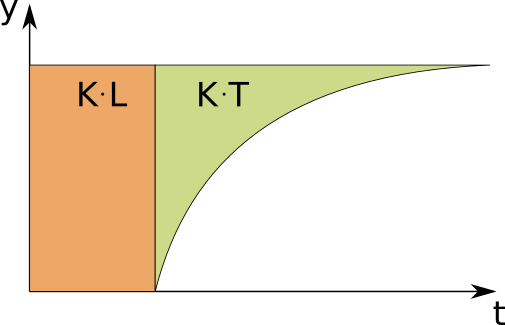
\includegraphics[width=0.9\textwidth]{./Graphics/AREA_IDENTIFICATION1.png}
\caption{Graphical Reprensentation of Identification via Jump Response}
\label{c:control:f:2area}
\end{minipage}
\end{figure}

\section{Controller Design}\label{c:control:s:identification}

The controller design can be divided into the SISO design process for a single controller and the MIMO design process for the interconnected system. Both tasks are equally important and are studied extensively throughout literature, see e.g. \cite{Astrom2000a}.\\

HERE SISO DESIGN PROCESS - MIGO, AMIGO, ROBUSTNESS ETC \\

\begin{figure}[H]
\begin{minipage}[b]{\textwidth}
\centering
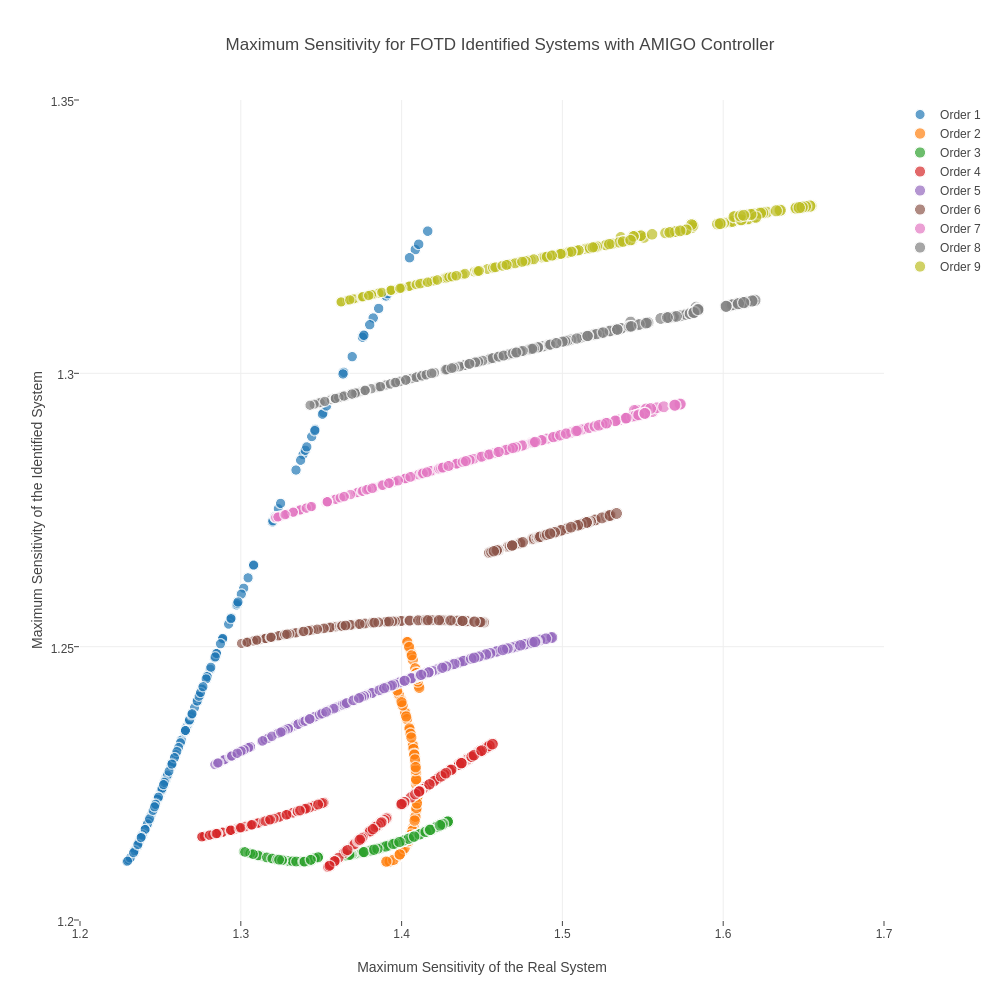
\includegraphics[width=0.9\textwidth]{./Graphics/PT9-Study.png}
\caption{Results of the Robustness Study, Maximum Sensitivity of the Real System and the Identified System}
\label{c:control:f:robustness_study}
\end{minipage}
\end{figure}

\section{Controller Design for Simple Process Models}

\subsection*{Relative Gain Array}
To design a set of controllers for the overall system several methods exist HAGGALUND, \cite{Skogestad2005MultivariableDesign}. A standard in industry is based on the Relative Gain Array (RGA) Analysis \cite[p.88 ff.]{Skogestad2005MultivariableDesign}.
The RGA is defined as

\begin{align}
\begin{split}
RGA\left(\ma{G}\right) &= \ma{G} \ma{G}^{-T} \\
&= \Lambda \left(\ma{G}\right) 
\end{split}
\label{c:control:e:RGA}
\end{align}

Eq. \ref{c:control:e:RGA} $\Lambda \in \mathbb{R}^{m \times l}$ provides a measure for the interaction of a control system at a specified frequency, most often the steady state of the system $s=0$ or the crossover frequency $s=\omega_0$.\newline
The controller synthesis based on the RGA is used extensively throughout industry, since it is an established, well known tool easy to understand.\newline
To give a better understanding, a TITO system is given explicitly by:

\begin{align}
\begin{split}
\Lambda \left( \ma{G} \right) &= \ma{G} \ma{G}^{-T} \\
&= \ma{G} \frac{1}{\det{\ma{G}}} \left[ tr\left( \ma{G} \right)\ma{I} - \ma{G} \right]^T  \\
&= \frac{tr \ma{G} }{\det \ma{G}} \ma{G} - \ma{G}\ma{G}^T \\  
\end{split}
\end{align}

The influence of each main input output pairing is reduced by the influence of other inputs acting on the desired output and the influence of this output on other inputs. A good way to visualize this is to multiply each element with the inverse product of the main diagonal Transfer Function $\frac{U_1}{Y_1} \frac{U_2}{Y_2}$, e.g. $\left( \frac{Y_1}{U_1}^2 - \frac{Y_1}{U_2}\frac{Y_2}{U_1} \right) \frac{U_1}{Y_1} \frac{U_2}{Y_2} = \frac{Y_1}{Y_2} \frac{U_2}{U_1} -1 = \frac{g_{11}}{g_{22}} -1$. If the resulting value is nearly 1, it follows that $g_{22} > g{11}$. This statement can be interpreted as recommendation to use the main couplings as pairings. \\

\section{Decoupling of Transfer Function Matrices}

\subsection*{Decoupling Control proposed by Astrom et.al.}
A method for the design of decoupling controllers is proposed in \cite{Astrom2001a} and \cite{Astrom2006AdvancedControl}. It designs a controller which limits the interaction near the steady state of the plant. To achieve this behaviour a decoupler $\ma{D} \in  \mathbb{R}^{n_y \times n_y}$ is introduced. A static decoupling is proposed such that $\ma{D} = \ma{G}^{-1}|_{s=0}$ that transforms the system with the mapping $\ma{G} \ma{D} = \ma{G}^* \in \mathbb{R}^{n_y \times n_y}$. The resulting closed loop is then given by: 

\begin{align}
\begin{split}
\ma{H} &= \left[ \ma{I}  - \ma{G} \ma{D} \ma{K}_y^* \right]^{-1} \ma{G} \ma{D} \ma{K}_r^* \\
	 &= \left[ \ma{I}  - \ma{G}^* \ma{K}_y^* \right]^{-1} \ma{G}^* \ma{K}_r^* \\
     &= \left[ \ma{I}  - \ma{G} \ma{K}_y \right]^{-1} \ma{G} \ma{K}_r \\
\end{split}
\label{c:control:e:closedloopastrom}
\end{align}
\nomenclature{$\ma{H}$}{Closed Loop Transfer Function}

Eq. \ref{c:control:e:closedloopastrom} gives various important transformations between the controller and system of the original identified system and the new transformed system. \\ 

A Taylor series around the steady state of the  transformed system is given by:

\begin{align}
\begin{split}
\ma{G}^* &= \sum_{i=0}^\infty \frac{d^i}{ds^i} \ma{G}^* |_{s=0} \frac{s}{i!} \\
&= \ma{I} + s \ma{\Gamma}^* + \ma{\mathcal{O}}\left(s^2\right) \\
&\approx \ma{I} +  \ma{\Gamma}^* s \\
&\approx \ma{I} + \left( \ma{\Gamma}^*_D + \ma{\Gamma}^*_A \right) s
\end{split}
\label{c:control:e:taylor}
\end{align}

In Eq.\ref{c:control:e:taylor} the coupling for small frequencies can be described via the coupling matrix $\ma{\Gamma}^* = \left( \gamma_{ij}^* \right)\in \mathbb{R}^{n_y \times n_y}$. The matrix consists both of diagonal and anti diagonal entries $\ma{\Gamma}^* = \ma{\Gamma}^*_D + \ma{\Gamma}^*_A$ which describe the small signal behaviour in an adequate way. \newline

Substitute Eq.\ref{c:control:e:taylor} in the numertator of Eq. \ref{c:control:e:closedloopastrom} holds:

\begin{align}
\begin{split}
\ma{H} &\approx \left[ \ma{I}  - \ma{G}^* \ma{K}_y^* \right]^{-1} \left[ \ma{I} +  \ma{\Gamma}^* s \right] \ma{K}_r^* \\
  &\approx \left[ \ma{I}  - \ma{G}^* \ma{K}_y^* \right]^{-1} \left[ \ma{I} + \left( \ma{\Gamma}^*_D + \ma{\Gamma}^*_A \right) s\right] \ma{K}_r^* \\
\end{split}
\end{align}

The anti diagonal entries are given by

\begin{align}
\begin{split}
\ma{H}_A &\approx \left[ \ma{I}  - \ma{G}^* \ma{K}_y^* \right]^{-1} \left[\ma{\Gamma}_A^* s \right] \ma{K}_r^*
\end{split}
\end{align}

Which is simplified according to Aström Paper to:

\begin{align}
\begin{split}
|h_{ij}| &= \left|\left(\prod_{k = 1}^{i} S_{k}^*\right)\gamma_{ij}^*s ~k^*_{r,jj} \right| \\
\end{split}
\label{c:control:e:interaction}
\end{align}

Where $k^*_{r,jj}$ is the j-th entry of the diagonal controller used for the reference signal $\ma{K}_r^*$. Eq. \ref{c:control:e:interaction} can be used to describe a decoupling of the controller by using an upper limit $h_{ij,max}^* \geq |h_{ij}^*| \in \mathbb{R}^+$ which describes the maximal allowed or desired interaction between the j-th input and the i-th output. For the special case where $k^*_{r,jj}$ is a pure integrator $k_{r,jj}^* = \frac{k_{I,jj}^*}{s}$ Eq. \ref{c:control:e:interaction} becomes:

\begin{align}
\begin{split}
\left| h_{ij} \right| &= \left|\left(\prod_k S_k^*\right) \gamma^*_{ij}~ k^*_{I,jj} \right| \\
& \leq \left|\left(\prod_k M_{S,k}^*\right) \gamma^*_{ij}~ k^*_{I,jj} \right| \\
& \leq \left|h_{ij,max}\right|
\end{split}
\label{c:control:e:setpointinteraction}
\end{align}

The relation given by Eq. \ref{c:control:e:setpointinteraction} gives a condition for detuning a purely integral controller. Since not every controller is given in this form, the structure is extended to PI control by:

\begin{align}
\begin{split}
\left|h_{ij}\right| &\leq \left| \left(\prod_k M_{S,k} \right) \gamma_{ij}^* s \left(k_{P,jj}^* + k_{I,jj}^* \frac{1}{s} \right) \right| \\
&\leq \left| \left(\prod_k M_{S,k} \right) \gamma_{ij}^*\right| \left|\left(k_{P,jj}^* s+ k_{I,jj}^* \right) \right| \\
&\leq \left| \left(\prod_k M_{S,k} \right) \gamma_{ij}^*\right| \left|\left(k_{P,jj}^* j\omega+ k_{I,jj}^* \right) \right| \\
&\leq \left| \left(\prod_k M_{S,k} \right) \gamma_{ij}^*\right| \sqrt{\left(k_{P,jj}^*\omega\right)^2+ \left(k_{I,jj}^*\right)^2} \\
\end{split}
\label{c:control:e:TransformedPIDetuning}
\end{align}

In Eq.\ref{c:control:e:TransformedPIDetuning} the influence of the proportional controller is increasing with the frequency. To detune the controller sufficiently, an adequate frequency must be chosen. For a small signal interpretation $\omega \ll 1$ a detuning for just the integral gain is acceptable.\\

In \cite[p.172 f.]{Skogestad2005MultivariableDesign} the crossover frequency of a transfer function is limited by an upper bound

\begin{align}
\omega_C &\leq \frac{1}{L}
\end{align}

Hence, an appropriate conservative boundary can be established with the minimum time delay of the system $L_{Min} | L\geq L_{Min} \forall L \in \Sigma $ to be:

\begin{align}
\begin{split}
\left| h_{ij} \right| &\leq \left| \left(\prod_k M_{S,k} \right) \gamma_{ij}^*\right| \sqrt{\left(\frac{k_{P,jj}^*}{L_{Min}}\right)^2+ \left(k_{I,jj}^*\right)^2}
\end{split}
\label{c:control:e:conservativePITuning}
\end{align}

Both Eq. \ref{c:control:e:setpointinteraction} and \ref{c:control:e:conservativePITuning} can be rewritten with a matrix $\ma{H}_{Max} = \left(h_{ij,Max}\right) \in \mathbb{R}^{n \times n}$ and the matrix of the maximum sensitivities of the diagonal transfer functions $\ma{M}_S^* = \left(M_{S,i}^*\right) \in \mathbb{R}^{n \times n}$. Using the definition of the maximum sensitivity matrix as diagonal, one can rewrite $\prod_k M_{S,k}^* = \det(\ma{M}_S) $. Once again dividing into a diagonal and anti diagonal matrix holds:

\begin{align}
\begin{split}
\ma{H}_{A,max} &\geq \det(\ma{M}_S^*) \ma{\Gamma}_A^* \ma{K}_r^* 
\end{split}
\label{c:control:e:Hmax*}
\end{align}



The method proposed above gives many advantages over a controller design based on RGA while holding the number of controllers minimal. The enhancement of performance comes through the interconnection of the controller outputs via the decoupler, which can be viewed as a simple form of model based control. Whilst giving major performance improvements, the presented method has a significant disadvantages.\\ 

Depending on the model chosen for identification and the values of the coefficients, the resulting transfer function will in general be of other form than the initial identified model. Hence, algorithms depending on these models to design controllers can not be used naturally, but have to use a simplified or approximated model. This process results in a higher model error and thus in poor performance and robustness of the derived controller.

\subsection*{Modified Controller Design Based on Astrom et.al.}

Because of these major penalties, a modified decoupling scheme is proposed. Essentially another interpretation of the equations given above leds to a more physical meaningful design process. At first, diagonal and anti-diagonal entries of a matrix multiplication are reviewed:

\begin{align}
\begin{split}
\ma{G}^{A} \ma{G}^{B} &= 
\begin{bmatrix}
\ma{G}_{11}^{A} & \ma{G}_{12}^{A} \\
\ma{G}_{21}^{A} & \ma{G}_{22}^{A} 
\end{bmatrix}
\begin{bmatrix}
\ma{G}_{11}^{B} & \ma{G}_{12}^{B} \\
\ma{G}_{21}^{B} & \ma{G}_{22}^{B} 
\end{bmatrix}\\
&= \begin{bmatrix}
\ma{G}_{11}^{A}\ma{G}_{11}^{B} + \ma{G}_{12}^{A}\ma{G}_{21}^{B} & \ma{G}_{11}^{A}\ma{G}_{12}^{B} + \ma{G}_{12}^{A}\ma{G}_{22}^{B} \\
\ma{G}_{21}^{A}\ma{G}_{11}^{B} + \ma{G}_{22}^{A}\ma{G}_{21}^{B} &
\ma{G}_{21}^{A}\ma{G}_{12}^{B} + \ma{G}_{22}^{A}\ma{G}_{22}^{B}
\end{bmatrix}
\end{split}
\label{c:control:e:matrixmult}
\end{align}

Eq. \ref{c:control:e:matrixmult} states that the diagonal entries relate to either pure diagonal or pure anti-diagonal entries of the factors. Anti-diagonal entries are always the mixed product of diagonal and anti-diagonal terms.\\

Starting with Eq. \ref{c:control:e:closedloopastrom} diagonal and antidiagonal entries of the numerator can be identified:

\begin{align}
\begin{split}
\ma{D}\ma{K}^* &= \ma{K} \\
\left(\ma{D}_D + \ma{D}_A \right) \ma{K}^* &= \left(\ma{K}_D + \ma{K}_A \right)\\
\left(\ma{D}_D + \ma{D}_A \right) \ma{D}^{-1} \ma{K} &= \left(\ma{K}_D + \ma{K}_A \right)
\end{split}
\label{c:control:e:eqscontroller}
\end{align}

Eq. \ref{c:control:e:eqscontroller} relates the diagonal controller $\ma{K}_D \in \mathbb{C}^{n \times n}$ designed via the diagonal transfer functions $g_{ii}$  to the decoupling controller proposed by Astr\"om et.al.. Since $\ma{K}^{*}$ is diagonal a direct relationship between the antidiagonal elements of the controller can be established:

\begin{align*}
\begin{split}
\ma{K}_A &= \ma{D}_A \ma{K}^* \\
&= \ma{D}_A D^{-1} \left( \ma{K}_D + \ma{K}_A \right) \\
\end{split}
\end{align*}

Which is able to relate the diagonal and antidiagonal controller to each other:

\begin{align}
\begin{split}
\ma{K}_A &= \left[ \ma{I} - \ma{D}_A \ma{D}^{-1} \right]^{-1} \ma{D}_A \ma{D}^{-1} \ma{K}_D \\
&= \left[\ma{D} \ma{D}_D^{-1} - \ma{I} \right] \ma{K}_D \\
&= \ma{D}_A \ma{D}_D^{-1} \ma{K}_D \\
&= \ma{\Sigma} \ma{K}_D
\end{split}
\label{c:control:e:splitter}
\end{align}

Eq. \ref{c:control:e:splitter} defines the splitter $\ma{\Sigma} \in \mathbb{R}^{n \times n}$ which can substitute the antidiagonal controller in Eq.\ref{c:control:e:eqscontroller}:

\begin{align}
\begin{split}
\ma{D} \ma{K}^* &= \left[ \ma{I} + \ma{\Sigma} \right] \ma{K}_D
\end{split}
\label{c:control:e:controleqs}
\end{align}

An interesting property of the splitter is the intuitive relation between the main diagonal entries of the system and the anti diagonal entries. Since we can invert a block sufficient conditioned block matrix via:

\begin{align}
\begin{split}
\begin{bmatrix}
\ma{G}_{11} & \ma{G}_{12} \\
\ma{G}_{21} & \ma{G}_{22} 
\end{bmatrix}^{-1} &= \begin{bmatrix}
\left[\ma{G}_{11} - \ma{G}_{12}\ma{G}_{22}^{-1}\ma{G}_{22}\right]^{-1} & -\ma{G}_{11}^{-1}\ma{G}_{12}\left[\ma{G}_{22} - \ma{G}_{21}\ma{G}_{11}^{-1}\ma{G}_{12}\right]^{-1}  \\
-\ma{G}_{22}^{-1}\ma{G}_{21}\left[\ma{G}_{11} - \ma{G}_{12}\ma{G}_{22}^{-1}\ma{G}_{21}\right]^{-1}  & \left[\ma{G}_{22} - \ma{G}_{12}\ma{G}_{11}^{-1}\ma{G}_{12}\right]^{-1} 
\end{bmatrix} \\
\end{split}
\end{align}

The splitter given by $\ma{D}_A\ma{D}_D^{-1}$ becomes in the notation above
\begin{align}
\begin{split}
\ma{\Sigma} &= \begin{bmatrix}
0 & -\ma{G}_{11}^{-1}\ma{G}_{12}\\
-\ma{G}_{22}^{-1}\ma{G}_{21}  & 0
\end{bmatrix}
\end{split}
\end{align}

It is clearly visible that the splitter weights the minor with the main diagonals. It can be connected both to feedforward control and disturbance rejection by dividing the system as shown in FIGURE.\\

Investigating the relationship between the diagonal Sensitivity of the transformed System and the ideal Sensitivities of the Diagonal system holds:

\begin{align}
\begin{split}
S^* &= \left[\ma{I}+\ma{G} \left[ \ma{I} + \ma{\Sigma} \right] \ma{K}_D \right]_D^{-1} \\
&= \left[\ma{I}+\ma{G}_D \ma{K}_D + \ma{G}_A \ma{\Sigma} \ma{K}_D  \right]^{-1} \\
&= \left[ \ma{S}^{-1} + \ma{\Delta}_{S}\right]^{-1}
\end{split}
\label{c:control:e:sensitivityerror}
\end{align}

Eq. \ref{c:control:e:sensitivityerror} states that the transformed sensitivity is not equal to the sensitivity of the main diagonal system. Instead an error $\ma{\Delta}_{S} \in \mathbb{C}^{n \times n}$ relating to the influence of the anti diagonal entries via feedback is formed. From Eq. \ref{c:control:e:sensitivityerror} follows directly

\begin{align}
\begin{split}
\ma{S} &= \left[ \ma{S}^{-*}- \ma{\Delta}_{S}\right]^{-1} \\
&= \left[ \ma{S}^{-*}\left[ \ma{I} - \ma{S}^{-*}\ma{\Delta}_S\right] \right]^{-1} \\
&= \left[ \ma{I} - \ma{S}^{-*}\ma{\Delta}_S\right]^{-1} \ma{S}^{*}
\end{split}
\label{c:control:e:sensitivitysolve}
\end{align}

Eq. \ref{c:control:e:sensitivitysolve} states equivalently

\begin{align}
\begin{split}
\ma{M}_S &\geq \ma{S} \\
&\geq \left[ \ma{I} - \ma{S}^{-*}\ma{\Delta}_S\right]^{-1} \ma{S}^{*}
\end{split}
\label{c:control:e:sensitivitytransform}
\end{align}

Eq. \ref{c:control:e:sensitivitytransform} describes the transformation between the Maximum Sensitivities. 
Using the Triangle inequality holds:

\begin{align}
\begin{split}
\left[\left| \ma{I} - \ma{S}^{-*} \ma{\Delta}_S  \right| \right]^{-1} &\geq \left[\ma{I} + \left|\ma{S}^{-*} \right| \left| \ma{\Delta}_S  \right| \right]^{-1} \\
&\geq \left[\ma{I} + \ma{M}_S^{-*} \left| \ma{\Delta}_S  \right| \right]^{-1} 
\end{split}
\end{align}

Hence, a conservative lower and upper bound can be defined:

\begin{align}
\begin{split}
\left[\ma{I} + \ma{M}_S^{-*} \min_\omega \left|\ma{\Delta}_{S}\right| \right]^{-1} \ma{M}_S^{*}\leq \ma{M}_S \leq 
\left[\ma{I} + \ma{M}_S^{-*} \max_\omega \left|\ma{\Delta}_{S}\right| \right]^{-1} \ma{M}_S^{*}
\end{split}
\label{c:control:e:sensitivitytransformBounds}
\end{align}

The lower boundary represents a conservative transformation. The most conservative transform is given by $\ma{\Delta}_S = \ma{0}$. This resembles the fact that the magnitude of superpositioned transfer functions is less or equal to the sum of its magnitudes. Hence, the most conservative approximation is given by assuming the system is equal to its transformed system. \\

To detune the controller the anti diagonal parts of the transfer function are used. Explicitly the term is given by

\begin{align}
\begin{split}
\ma{\Gamma}_A &= \left[\frac{d}{ds}\left[ \ma{G} \left[ \ma{I} + \ma{\Sigma} \right] \right]|_{s=0}\right]_A\\
&= \frac{d}{ds}\left[ \ma{G}_A + \ma{G}_D \ma{\Sigma} \right]|_{s=0}
\end{split}
\end{align}

With the maximum allowed interaction and sensitivities the detuning formula is given by:

\begin{align}
\begin{split}
\ma{H}_{A,Max} &\geq \ma{M}_S \ma{\Gamma}_A \ma{K}_r \\ 
&\geq \det(\ma{M}_S) \ma{\Gamma}_A \ma{K}_r 
\end{split}
\end{align}


\chapter{Control of Common Examples}
\label{c:examples}

The folllowing chapter 

\section{Decoupling of FOTD Process Models}
\label{c:examples:s:FOTD}

Since a FOTD are the model structure choosen for this work a deeper investigation of transfer function matrices based on this model is performed. For the following section a simple two input two output model given as following is defined:

\begin{align}
\begin{split}
\ma{G} = \begin{bmatrix}
g_{11} & g_{12} \\
g_{21} & g_{22}
\end{bmatrix} & ~,g_{ij} = \frac{K_{ij}}{T_{ij} s +1 } e^{-L_{ij}s}
\end{split}
\label{c:examples:e:examplesys}
\end{align}

For the system described in Eq. \ref{c:examples:e:examplesys} three different controller based on PI-structure are defined using the methods presented in the previous chapter. Further restrictions on the systems performance are given by the Maximum Sensitivity and Maximum Interaction of the system given by:

\begin{align}
\begin{split}
\ma{H}_{A,Max} &= \begin{bmatrix}
0 & h_{12,Max} \\
h_{21,Max} & 0 
\end{bmatrix}\\
\ma{M}_{S} &= \begin{bmatrix}
M_{S,1} & 0 \\
0 & M_{S,2}
\end{bmatrix}
\end{split}
\label{c:examples:e:restrictions}
\end{align}

Eq.\ref{c:examples:e:restrictions} is given under the assumption that only the diagonal transfer functions are requiered and the interaction acts on the antidiagonal entries. Furthermore the system will be operating near steady state and hence the frequency used for Taylor Series Exapnsion is choosen to be $s = 0$.

\subsection*{Controller Design via Relative Gain Array Analysis}

Assuming the diagonal dominance of the system, the controller are designed via the transfer functions $g_{11}$ and $g_{22}$. Since the AMIGO Algorithm has been given earlier ZITIEREN and explicit values for this example will be given later on, no further description will be given at this point.


\subsection*{Controller Design via Astr\"om et. al.}

At first the decoupler is designed via the inverse static gain of the system


\begin{align}
\begin{split}
\ma{D} &= \ma{G}|_{s=0}^{-1}\\
&= \frac{1}{K_{11}K_{22}-K_{12}K_{21}} 
\begin{bmatrix}
K_{22} & -K_{21} \\
-K_{12} & K_{11}
\end{bmatrix}
\end{split}
\label{c:examples:e:exampleDecoupler}
\end{align}

And with the decoupler the transformed system $\ma{G}^*$ is calculated to be

\begin{align}
\begin{split}
\ma{G}^* &= \ma{G}\ma{D}\\
&= \frac{1}{K_{11}K_{22}-K_{12}K_{21}} 
\begin{bmatrix}
g_{11} & g_{12} \\
g_{21} & g_{22}
\end{bmatrix}
\begin{bmatrix}
K_{22} & -K_{21} \\
-K_{12} & K_{11}
\end{bmatrix} \\
&= \frac{1}{K_{11}K_{22}-K_{12}K_{21}}
\begin{bmatrix}
K_{22}g_{11}-K_{12}g_{12} & -K_{21}g_{11}+K_{22}g_{12} \\
K_{22}g_{21}-K_{12}g_{22} &
-K_{21}g_{21}+K_{11}g_{22}
\end{bmatrix}
\end{split}
\label{c:examples:e:exampletransformed}
\end{align}

From Eq. \ref{c:examples:e:exampletransformed} it is clear that the entries $g_{ij}^*$ are linear combinations of FOTD transfer functions. Due to the properties of the exponential function the superposition principle does not hold. Hence a controller via the AMIGO algorithm can only be designed if a sufficient approximation of the linear combination as a FOTD can be formulated:

\begin{align}
\begin{split}
g_{ij}^* & = \frac{K_{ij}^*}{T_{ij}^*s+1}e^{-L_{ij}^* s} + \Delta g_{ij}^*\\
&\approx \frac{K_{ij}^*}{T_{ij}^*s+1}e^{-L_{ij}^* s} 
\end{split}
\label{c:examples:e:exampleFOTDapprox}
\end{align}

Within Eq. \ref{c:examples:e:exampleFOTDapprox} the main drawback of the method is layed out. As stated earlier, most algorithms for PI(D) design rely on a fixed model structure and hence are not fit to process information given by a combination. To use the function, two methods are proposed.\\

Assuming the results of the experiment used for identifying the process are still avaible the process approximate model can be found via a weighted sum of the systems output. First the static gain of every transfer function is determined via

\begin{align}
\begin{split}
K_{ij} &= \frac{y_{i}(\infty) - y_{i}(0)}{u_{j}(\infty)-u_j(0)}
\end{split}
\label{c:examples:staticgain}
\end{align}

As explained earlier. Subsequent the results of a linear combination are given by:

\begin{align}
\begin{split}
y_{1}^*(t) &= \frac{K_{22} y_{11}(t) - K_{12} y_{12}(t)}{\det(\ma{K})}
\end{split}
\label{c:examples:e:Combination}
\end{align}

Eq. \ref{c:examples:e:Combination} reuses the experimental data to approximate the systems output. $y_{ii}$ is the i-th output of the system reacting to excitation via the i-th input. Hence the data can be used for FOTD identification as presented earlier.\\

The second method relies on knowledge about the behaviour of the transfer functions in the time domain. At first, the static gain is given by:

\begin{align}
\begin{split}
K_{11}^* &= \frac{K_{22} K_{11} - K_{12}^2}{\det(K)}
\end{split}
\label{c:examples:e:CombinationGain}
\end{align}

Since the integral is a linear operator the time integral can be rewritten as:

\begin{align}
\begin{split}
\int_0^\infty y_{1}^*(\infty) - y_1^*(t) dt &= K_{11}^* (T_{11}^*+L_{11}^*) \\
&= \frac{1}{\det(K)} \left( K_{22} \int_0^\infty y_{11}(\infty) - y_{11}(t) dt + K_{12} \int_0^\infty y_{12}(\infty) - y_{12}(t) dt\right) \\
&= \frac{1}{\det(K)} \left( K_{22} K_{11} (T_{11}+L_{11}) + K_{12}^2 (T_{12}+L_{12}) \right) 
\end{split}
\label{c:examples:e:CombinationIntegral}
\end{align}

To determine the coefficients of the new system a third equation is needed. It is convinient to choose an appropriate value for the new time delay $L^*$ with several options like a weighted sum, the minimum or maximum of all involved delays. A robust method is given by choosing the maximum and hence implement a conservative tuning. Subsequently Eq. \ref{c:examples:e:CombinationIntegral} can be rearranged to

\begin{align}
\begin{split}
T_{11}^* &= \frac{1}{\det(K)K_{11}^*} \left( K_{22} K_{11} (T_{11}+L_{11}) + K_{12}^2 (T_{12}+L_{12}) \right) - L_{11}^*
\end{split}
\label{c:examples:e:CombinationTimeConstant}
\end{align}

Assuming a sufficient approximation can be found and the resulting error is minimal the diagonal controller can be designed. A choice for a PI-Structure with set point weighting $b=0$ holds:

\begin{align}
\begin{split}
\ma{K}_y^* &= \begin{bmatrix}
-K_{P1}^* - K_{I1}^*\frac{1}{s} & 0 \\
0 & -K_{P2}^* - K_{I2}^*\frac{1}{s}
\end{bmatrix} \\
\ma{K}_r^* &= \begin{bmatrix}
K_{I1}^*\frac{1}{s} & 0 \\
0 & K_{I2}^*\frac{1}{s}
\end{bmatrix} 
\end{split}
\label{c:examples:e:exampleTransformedControler}
\end{align}

With parameters $K_{P,i},K_{I,i} \in \mathbb{R}$ are calculated via the AMIGO Tuning Rules as given earlier. Since the approximation given in Eq.\ref{c:examples:e:exampleFOTDapprox} holds an inevitable error so do the parameter. \\

The coupling matrix of the antidiagonal parts is given by:

\begin{align}
\begin{split}
\ma{\Gamma}_A &= \left[\frac{d}{ds}\ma{G}|^*_{s=0}\right]_A s \\
&= \begin{bmatrix}
0 & \frac{-K_{21}K_{11}(T_{11}-L_{11}) + K_{22}K_{12}(T_{12}-L{12})}{K_{11}K_{22}-K_{12}K_{21}} \\
\frac{-K_{12}K_{22}(T_{22}-L_{22}) + K_{22}K_{21}(T_{21}-L_{21})}{K_{11}K_{22}-K_{12}K_{21}} & 0
\end{bmatrix} s\\
&\approx \begin{bmatrix}
0 & K_{12}^* (T_{12}^* - L_{12}^*) \\
K_{21}^* (T_{21}^* - L_{21}^*) & 0 
\end{bmatrix} s
\end{split}
\label{c:examples:e:exampleTransformedCoupling}
\end{align}

From Eq. \ref{c:examples:e:exampleTransformedCoupling} the dependency of the coupling on the both the static gain of the system and the dynamical behaviour can be observed. This coincides with the statements of LUNZE ZITIEREN.\\

Detuning the controller requires to define both  maximum allowed interactions $h_{ij,Max}$ and maximum sensitivity $M_{S,i}$ of the closed loop:

\begin{align*}
\begin{split}
\ma{H}_{A,Max} &= \begin{bmatrix}
0 & h_{12,Max} \\
h_{21,Max} & 0 
\end{bmatrix}\\
\ma{M}_{S} &= \begin{bmatrix}
M_{S,1} & 0 \\
0 & M_{S,2}
\end{bmatrix}
\end{split}
\end{align*}

Solving Eq. \ref{c:examples:e:Hmax*} for the set point weighting controller holds:

\begin{align}
\begin{split}
\ma{K}^*_r &\leq \ma{\Gamma}^{-*}_{A,Max}\ma{M}_S^{-1}\ma{H}^*_{A,Max} \\ 
&\leq \frac{1}{\det(\ma{M}_S)}\ma{\Gamma}^{-*}_{A,Max}\ma{H}^*_{A,Max}\\
&\leq \frac{1}{M_{S,1}M_{S,2}}
\begin{bmatrix}
\frac{h_{21,Max}}{K_{12}^* (T_{12}^* - L_{12}^*)} & 0\\
0 & \frac{h_{12,Max}}{K_{21}^* (T_{21}^* - L_{21}^*)} 
\end{bmatrix}
\end{split}
\end{align}


\subsection*{Controller Design via Modified Astr\"om}

Now the modified Algorithm proposed in this thesis is applied to the same System. First, we design the controller as a function of the main diagonal entries $g_{ii}$ once again using the AMIGO Tuning rules:

\begin{align}
\begin{split}
\ma{K}_y &= \begin{bmatrix}
-K_{P1} - K_{I1}\frac{1}{s} & 0 \\
0 & -K_{P2} - K_{I2}\frac{1}{s}
\end{bmatrix} \\
\ma{K}_r &= \begin{bmatrix}
K_{I1}\frac{1}{s} & 0 \\
0 & K_{I2}\frac{1}{s}
\end{bmatrix} 
\end{split}
\label{c:examples:e:exampleControler}
\end{align}

The splitter $\ma{\Sigma}$ is likewise designed by the steady state of the system as:

\begin{align}
\begin{split}
\ma{\Sigma} &= \ma{D}_A\ma{D}_D^{-1} \\
& = \begin{bmatrix}
0 & -\frac{K_{12}}{K_{11}} \\
-\frac{K_{21}}{K_{22}} & 0
\end{bmatrix}
\end{split}
\end{align}

To test for interaction define the maximum interaction and the sensitivity like in Eq. FEHLT. The anti diagonal parts of the Taylor series can be identified as:

\begin{align}
\begin{split}
\ma{\Gamma}_A &= \frac{d}{ds}\left[\ma{G}_A + \ma{G}_D\ma{\Sigma}\right]|_{s=0} \\
&= \begin{bmatrix}
0 & K_{12}(T_{12}-L_{12}) - K_{11}\frac{K_{12}}{K_{11}}(T_{11}-L_{11}) \\
K_{21}(T_{21}-L_{21}) - K_{22}\frac{K_{21}}{K_{22}}(T_{22}-L_{22}) & 0 
\end{bmatrix} \\
&= \begin{bmatrix}
0 & K_{12}(T_{12}-L_{12} - T_{11}+L_{11}) \\
K_{21}(T_{21}-L_{21} - T_{22}+L_{22}) & 0 
\end{bmatrix} 
\end{split}
\end{align}

To detune the controller solving Eq. \ref{c:examples:e:Hmax*} for the integral controller as before holds:

\begin{align}
\begin{split}
\ma{K}_I &\leq \ma{\Gamma}_A^{-1} \ma{M}_S^{-1} \ma{H}_{A,Max} \\
&\leq \frac{1}{\det(\ma{M}_S)} \ma{\Gamma}_A^{-1} \ma{H}_{A,Max} \\
&\leq \frac{1}{M_{S,1}M_{S,2}}\begin{bmatrix}
\frac{h_{12,Max}}{K_{12}(T_{12}-L_{12}-T_{11}+L_{11})} & 0 \\
0 &\frac{h_{21,Max}}{K_{21}(T_{21}-L_{21}-T_{22}+L_{22})}
\end{bmatrix}
\end{split}
\end{align}
\subsection*{Overview}

Three Methods are presented above. 




%\chapter{Grundlagen}
\label{sec:Grundlagen}



\section{Wert und Einheit}
\label{sec:Unit}
Viele Einheiten lassen sich sch�ner darstellen mit dem Latex Befehl \verb|\unit[]{}| beziehungsweise \verb|\unitfrac[]{}{}|. Siehe den Vergleich: ohne 1~m oder mit \unit[1]{m} bzw. ohne 1~m/sec oder mit \unitfrac[1]{m}{sec}. Des weiteren kann zum Beispiel mit \verb|\textcelsius| ein \textcelsius{} Symbol eingef�gt werden.

\section{�berschrift}
\label{sec:Quelltext}
Text Text Text Text Text Text Text Text Text Text Text Text Text Text Text Text Text Text Text Text Text Text Text Text Text Text Text Text Text Text Text Text Text Text Text Text Text Text Text Text Text Text Text Text Text Text Text Text Text Text Text Text Text Text Text Text Text Text Text Text Text Text Text Text Text Text Text Text Text Text Text Text

\section{Abbildungen einbinden}
\label{sec:pictures}
Text Text Text Text Text Text Text Text Text Text Text Text Text Text Text Text Text Text Text Text Text Text Text Text Text Text Text Text Text Text Text Text Text Text Text Text Text Text Text Text Text Text Text Text Text Text Text Text Text Text Text Text Text Text Text Text Text Text Text Text Text Text Text Text Text Text Text Text Text Text Text Text Text Text Text Text Text Text 


\begin{figure}[htbp]
  \centering
  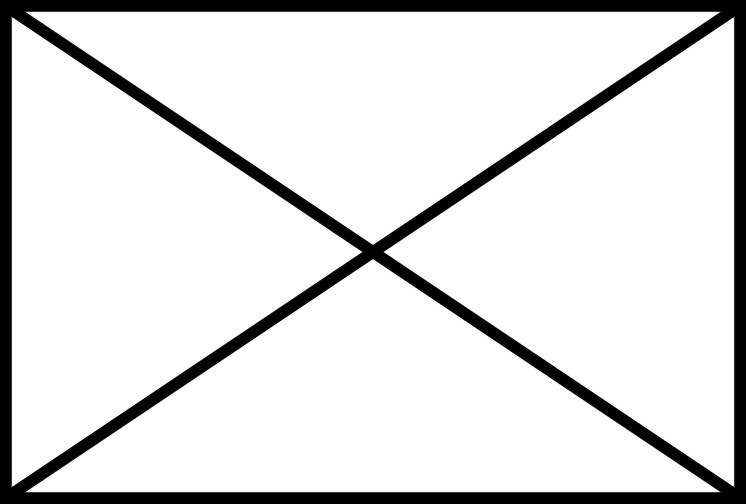
\includegraphics{pictures/empty.jpg}
  \caption{Einzelne Abbildung}
  \label{fig:singlepicture}
\end{figure}


Text Text Text Text Text Text Text Text Text Text Text Text Text Text Text Text Text Text Text Text Text Text Text Text Text Text Text Text Text Text Text Text Text Text Text Text Text Text Text Text Text Text Text Text Text Text Text Text Text Text Text Text Text Text Text Text Text Text Text Text Text Text Text Text Text Text Text Text Text Text Text Text Text Text Text Text Text Text Text Text Text Text Text Text Text Text Text Text Text Text Text Text Text Text Text Text Text Text Text Text Text Text Text Text Text Text Text Text Text Text Text Text Text Text Text Text Text Text Text Text Text Text Text Text Text Text Text Text Text Text Text Text Text Text Text Text Text Text Text Text Text Text Text Text Text Text Text Text Text 



Text Text Text Text Text Text Text Text Text Text Text Text Text Text Text Text Text Text Text Text Text Text Text Text Text Text Text Text Text Text Text Text Text Text Text Text Text Text Text Text Text Text Text Text Text Text Text Text Text Text Text Text Text Text Text Text Text Text Text Text Text Text Text Text Text Text Text Text Text Text Text Text Text Text Text Text Text Text Text Text Text Text Text Text Text Text Text Text Text Text Text Text Text Text Text Text Text Text Text Text Text Text Text Text Text Text Text Text Text Text Text Text Text Text Text Text Text Text Text Text Text Text Text Text Text Text Text Text Text Text Text Text Text 
%\addchap{Symbolverzeichnis}
\label{Symbolverzeichnis}

\begin{tabbing}
\hspace*{3.5cm}                              \=  \hspace*{10.0cm}                     \= \kill
\textbf{Formelzeichen}                       \> \textbf{Bedeutung}                    \> \textbf{Einheit} \\
~\\
${I}$                                        \> Strom                                 \> A  \\
${i}$                                        \> Getriebe�bersetzung                   \> -  \\
${l}$                                        \> L�nge                                 \> m  \\
${M}$                                        \> Drehmoment                            \> N  \\
${m}$                                        \> Masse                                 \> Kg \\
${n}$                                        \> Drehzahl                              \> 1/sec \\
${R}$                                        \> Widerstand                            \> $\Omega$ \\
${t}$                                        \> Zeit                                  \> sec \\
${U}$                                        \> Spannung                              \> V \\
~\\
${\alpha}$                           		 \> Drehwinkel von Gelenk 1               \> rad \\
${\beta}$                           	 	 \> Drehwinkel von Gelenk 2               \> rad \\
${\Delta \varepsilon}$   				 	 \> Aufl�sung der Drehwinkelsensoren      \> rad/Imp. \\
${\varepsilon}$                      		 \> Drehwinkel allgemein                  \> rad \\
${\theta}$              					 \> Tr�gheitsmoment                       \> Kg$\cdot$m$^2$ \\
~\\
~\\
\textbf{Indizes}                             \> \textbf{Bedeutung} \\
~\\
${0}$                                        \> Leerlauf \\
${el}$                                       \> elektrischer Teil der Motoren \\
${mech}$                                     \> mechanischer Teil der Motoren \\
${G}$                                        \> Getriebe \\
${i, j}$                                	 \> Laufindex (1, 2, 3, ...) \\
${Ref}$                                      \> Referenzwert \\
${soll}$                                     \> Sollgr��e \\
\end{tabbing}

\bibliography{chapters/mendeley_masterarbeit} 

\Anhang
\section{Erster Anhang}
\label{sec:Anhang_1}
Ein Anhang.


\section{Zweiter Anhang}
\label{sec:Anhang_2}
Ein weiterer Anhang.



%--------------------------------------------------
%--------------Ende eigener Kapitel----------------
%--------------------------------------------------

\makebackpage[trisec]%[<plain/info/addressinfo>]
\end{document}
